\documentclass[en,hazy,blue,screen,14pt]{elegantnote}
\usepackage[T1]{fontenc}
\usepackage[latin9]{inputenc}
\usepackage{babel}
\usepackage{float}
\usepackage{textcomp}
\usepackage{amsmath,amsfonts,amssymb}
\usepackage{amsthm}
\usepackage{graphicx}
\usepackage[ruled,vlined]{algorithm2e}
\PassOptionsToPackage{normalem}{ulem}
\usepackage{ulem}
\usepackage{mathtools}
\DeclarePairedDelimiter{\ceil}{\lceil}{\rceil}

\title{Class Notes\\CIS 502 Analysis of Algorihtm\\Week 4 - }
\author{Da Kuang}
\institute{University of Pennsylvania}
% \version{1.00}
\date{}

\begin{document}

\maketitle
\newpage
This week we talked about two more example about devide and conquer:
\begin{itemize}
 \item Polynomial Multiplication
 \item Convex Hulls on the Plane
\end{itemize}

\section{Polynomial Multiplication}
\subsection{Introduction}
A polynomial in the variable x over an algebraic field F represents a function 
$A(x)$ as a formal sum:
\[A(x) = \sum_{j = 0}^{n-1} a_j x^j\]
We call the values $a_0, ~a_1, ~\cdots, ~a_{n-1}$ the \textbf{coefficients} of 
the polynomial. The coefficients are drawn from a field $F$ , typically the set 
$\mathbb{C}$ of complex numbers. A polynomial can be represented as a list of 
coefficients in computer.

A polynomial $A(x)$ has \textbf{degree $k$} if its highest nonzero coefficient 
is $a_k$. we write that $\text{degree}(A) = k$. Any integer strictly greater 
than the degree of a polynomial is a \textbf{degree-bound }of that polynomial. 
Therefore, the degree of a polynomial of degree-bound $n$ may be any integer 
between $0$ and $n-1$, inclusive.

Polynomial Multiplication: if $A(x)$ and $B(x)$ are polynomials of degree-bound 
$n$, their product $C(x)$ is a polynomial of degree-bound $2n - 1$ such that
$C(x) = A(x)B(x)$ for all $x$ in the underlying field. For example,

\centerline{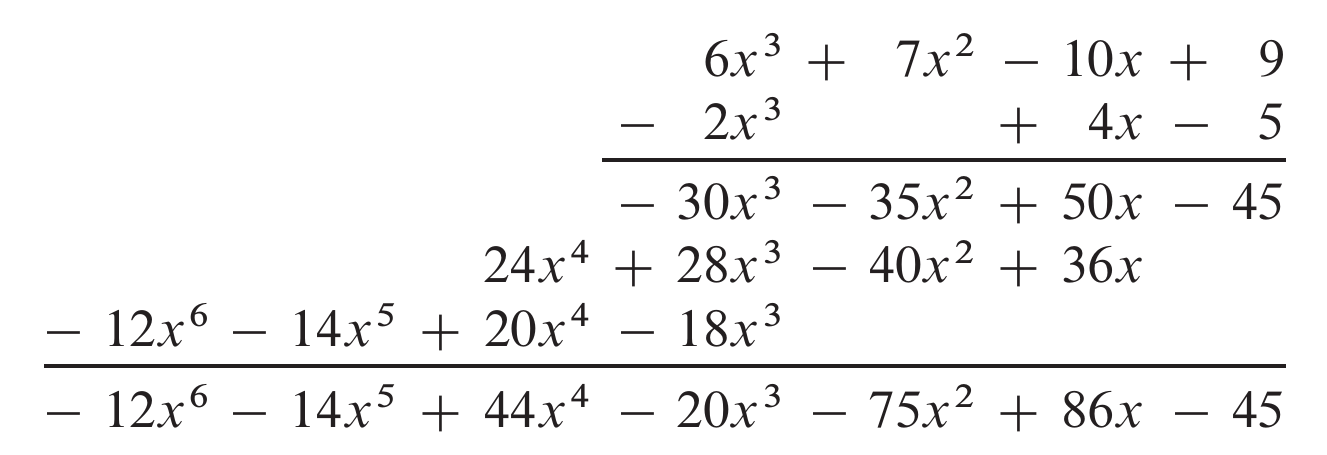
\includegraphics[width=0.5\textwidth]{poly-multiply.png}}

Another way to express the product $C(x)$ is
\begin{align*}
 C(x) = \sum_{j=0}^{2n-2} c_j x^j\\
 \intertext{where}
 c_j = \sum_{k=0}^j a_k b^{j-k}
\end{align*}

Note that $\text{degree}(C) = \text{degree}(A) +  \text{degree}(B)$, implying 
that if $A$ is a polynomial of degree-bound $n_a$ and $B$ is a polynomial 
of degree-bound $n_b$ , then $C$ is a polynomial of degree-bound $n_a + n_b - 
1$. Since a polynomial of degree-bound $k$ is also a polynomial of degree-bound 
$k + 1$, we will normally say that the product polynomial $C$ is a polynomial 
of degree-bound $n_a + n_b$.

\subsection{Algorithm}
Input: Two polynomials with same degree $d$:
\begin{align*}
 A &= a_d x^d + \cdots + a_0\\
 B &= b_d x^d + \cdots + b_0
\end{align*}
Goal: Calculate the product of the inputs.

\subsubsection{Baseline Method}
Simply calculate each parameter based on the definition of polynomial product. 
Each parameter in $A(x)$ should multiply all the parameters in $B(x)$ 
which takes $O(n^2)$ steps.
\subsubsection{Devide and Conquer}
\textbf{Assumption}: To make sure the parameters could be nicely divided by 
two, we assume the degree $d$ of both polynomials is always $2^k - 1$, where $k 
\in \mathbb{N}$.

Devide the $(d+1)$ entries of polynomials as follows to reduce the problem size:

\centerline{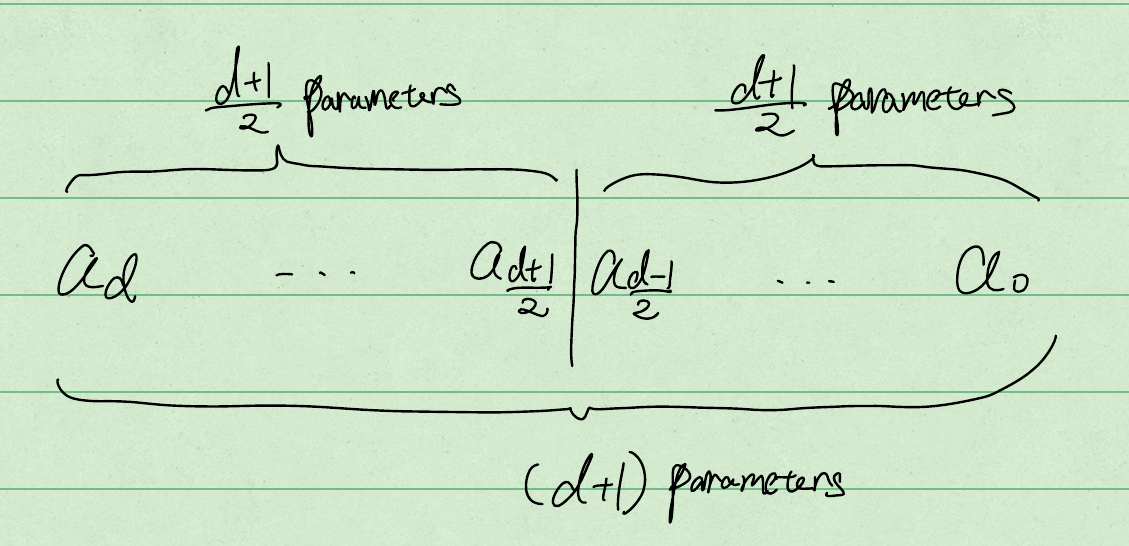
\includegraphics[width=0.5\textwidth]{poly-devide.png}}

Call the right hand side of polynomial as $A_l$. Extract $x^{\frac{d+1}{2}}$ 
and call the left hand side of polynomial as $x^{\frac{d+1}{2}} A_h$. we have,
\begin{align*}
 A &= x^{\frac{d+1}{2}} A_h + A_l\\
 B &= x^{\frac{d+1}{2}} B_h + B_l\\
 \intertext{Based on the algebra,}
 A \times B &= (x^{\frac{d+1}{2}} A_h + A_l)(x^{\frac{d+1}{2}} B_h + B_l)\\
 &= x^{d+1}A_h B_h + x^{\frac{d+1}{2}}A_h B_l + x^{\frac{d+1}{2}}A_l B_h + A_l 
B_l
\end{align*}
Therefore, we reduce the problem into four sub-problems with half of the size. 
Suppose the number of parameters is $n$, i.e. the degree of polynomials is $d = 
n - 1$. The reursion equation as follows:
\[T(n) \le 4T(\frac{n}{2}) + cn\]
Based on master theorem, $T(n) = O(n^2)$. Unfortunately, we have not get any 
improvement from those nicely splits comparing with the baseline. If you think 
about it, the result is actually not supring because even though the problem 
size is reudced, we could not skip any of the necessary multiplication. In 
other words, there are still $n^2$ necessary muliplications to get the 
production.

\textbf{Motivation}: When you have a recursive algorithm, saving  one operation 
could have a cascde effect and reduce the run time quickly. Adding polynomials 
only costs $O(n)$ steps. If we could reduce mutilication by addting addition. 
Then we are able to achieve better performance. 

To reduce the muliplications by adding additions, we have
\begin{align*}
 A \times B &= x^{d+1}A_h B_h + x^{\frac{d+1}{2}}A_h B_l + x^{\frac{d+1}{2}}A_l 
B_h + A_lB_l\\
            &= x^{d+1}A_h B_h + x^{\frac{d+1}{2}}(A_h B_l + A_l B_h) + A_l 
B_l
\end{align*}
Therefore, there are three items to calculate
\begin{enumerate}[(1)]
 \item $A_h B_h$
 \item $A_l B_l$
 \item $A_h B_l + A_l B_h$
\end{enumerate}
(1) and (2) are two muliplications. Moreover, (3) can be calculate by one more 
multiplication as follwing:
\begin{align*}
 &  (A_h + A_l) (B_h + B_l) - A_h B_h - A_l B_l\\
 =& A_hB_h + A_hB_l + A_lB_h + A_lB_l - A_h B_h - A_l B_l\\
 =& A_lB_h + A_lB_l
\end{align*}

Therefore, the recursive function becomes
\[T(n) \le 3T(\frac{n}{2}) + cn\]
It can be solved by master theorem, where $a = 3, b = 2, c = 1$.

Since $\log_ba > 1 = c$, so $T(n) = O(n^{\log_2 3}) \approx O(n^{1.6})$
\section{Convex Hull on the Plane}
\subsection{Introduction}
\subsubsection{Convex set}
Convex set A set $S \subseteq \mathbb{R}^n$ is said to be convex if $\forall 
x,y \in S$, the line segment joining $x$ and $y$ is contained in $S$.

\centerline{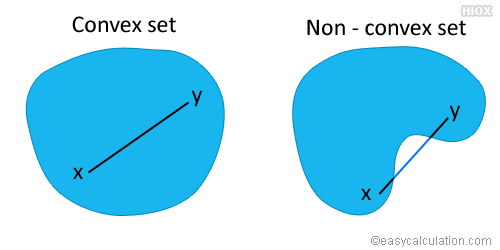
\includegraphics[width=0.5\textwidth]{convex-nonconvex-set.png}}
\subsubsection{Convex Combination}
Given two points $x=(x_1, x_2)$ and $y = (y_1, y_2) \in \mathbb{R}^2$, a convex 
combination of $x$ and $y$ is defined by
\[\lambda x + (1 - \lambda) y = \lambda x_1 + (1 - \lambda)y_1 + \lambda x_2 + 
(1 - \lambda)y_2, \text{ for } \lambda \in [0,1]\]
Changing the value of $\lambda$, we walk thought the segment. In general, 
 is the area confined by the edges formed by points.
\subsubsection{Convex Hull}
\textbf{Definition 1}: Convex hull of a finite set of points $S$ is the set of 
all points that can be expressed as convex combinations of points in $S$. 

\textbf{Definition 2}: Convex hull of a set of points is the smallest convex 
set that contains these points.
 
More intuitively, convex hull is like a rubber band streched from infinite and 
struck on the nails on points.
\centerline{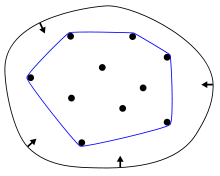
\includegraphics[width=0.5\textwidth]{ConvexHull.png}}
\subsubsection{Convex polygon}
Convex polygon is a polygon which is a convex set. It always contains interior 
angle which larger than 180 degree.
\subsection{Algorithm}
\begin{itemize}
 \item Input: $n$ points, $(x_1, y_1), (x_2, y_2), \cdots, (x_n, y_n)$.
 \item Output: The sequence of points on the boundary in counterclock order.
\end{itemize}

\subsubsection{Relative Location of Line and Points}
Given a line by two points $(x_1, y_1), (x_2, y_2)$ , a joining segment can 
be represented as follows:
\[y - y_1 = \frac{y_1 - y_2}{x_1 - x_2} (x - x_1)\]

For any third point $(x_3, y_3)$, it is possible determine which side of the 
line the third point lies. For instance, the thirds point is above the segment 
if 
\[y_3 - y_1 > \frac{y_1 - y_2}{x_1 - x_2} (x_3 - x_1)\]

\subsubsection{Convex Hull Successive Points Lemma}
\begin{itemize}
 \item If there is a segment joining two points such that all the other 
points lie on the same side of the segment, the segemnt represents two points 
on the convex hull.
 \item Conversely, if you have a segment on the convex hull and extending it, 
then every point from the convex hull will lie on the same side of the line.
\end{itemize}

\subsubsection{Baseline}
\begin{enumerate}
\item Use the extrem point as a start $x$.
\item Take every pair of points with $x$. write the equation for the line 
joining them and find the line where all other the points lie on the same side.
\item The line is a segment of convex hull.
\item Set $x$ to the other point of the segment and then repeat step 2.
\end{enumerate}

\paragraph{Runing Time Analysis}
\begin{itemize}
\item Determine all the points are on the same side of segemnt takes $O(n)$ 
steps.
\item To find one convex hull segment, we should check $O(n)$ segments.
\item There are at most $O(n)$ convex hull segemnt.
\item Therefore, the total run time is $O(n^3)$.
\end{itemize}

\subsubsection{Devide and Conquer}
Tips: To be efficient, we could like the sizes of sub-problems in devide and 
conquer to be same.

Devide points into those with $x$-corrdinates $\le x_{median}$ and those with 
$x$-corrdinates $> x_{mdian}$.



\end{document}
